\documentclass[english,svgnames,notes=hide,14pt]{beamer}
\usepackage{macros-ohp}
\usepackage{fontawesome}
\usepackage{lipsum}
\usepackage{multimedia}
\usepackage{setspace}
% \usepackage{media9}
\usepackage{graphicx}



\def\presentationtitle{Lindsey the Tour Guide Robot }

\title{\presentationtitle}
\author[N. Surname]{{Name Surname} \\*
    {\footnotesize\faEnvelope \, \texttt{nsurname@lincoln.ac.uk}}
}
\institute{\faInstitution \, Lincoln Centre for Autonomous Systems, UoL, UK}

%Please make sure the tex is compiled twice to have all the images displayed correctly.

%Fill the date or leave it blank to not display it
\date[L-CAS Away Day, Sept 2019]{\textbf{L-CAS away day}, somewhere in Lincoln,\\ September 2019}


\begin{document}

 %put [plain] at the end to get rid of the page number on this page
\begin{frame}[plain, noframenumbering]
  \titlepage
\end{frame}


\begin{frame}[noframenumbering]{Presentation Content}
    \tableofcontents
\end{frame}

\section{Project Overview}

\begin{frame}{The project}
    \begin{textblock*}{7cm}(5.5cm,0.5cm)
    \begin{block}{Lindsey the robot} % {block width} (coords)
    Autonomous robot that gives guided tours and information to the public at The Collection Museum in Lincoln.
    \end{block}
    \end{textblock*}
   
    \begin{textblock*}{7.5cm}(5cm,3cm) % {block width} (coords)
    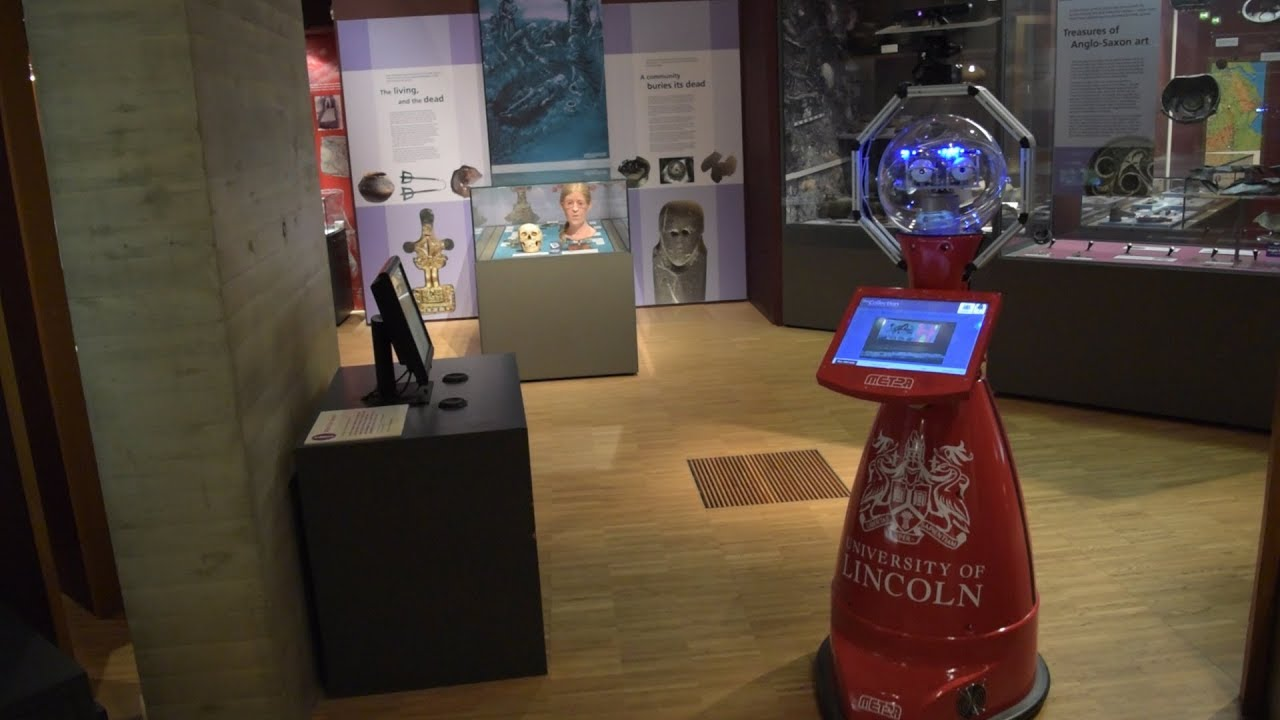
\includegraphics[width=\linewidth]{imgs/lindsey.jpg}
    \end{textblock*}
    \begin{textblock*}{4.4cm}(0.5cm,1.5cm) % {block width} (coords)
    \includegraphics[width=\linewidth]{example-image-b}
    \end{textblock*}
     \begin{textblock*}{3cm}(5.4cm,6.1cm) % {block width} (coords)
    \includegraphics[width=\linewidth]{example-image-c}
    \end{textblock*}
    \begin{textblock*}{3.5cm}(0.8cm,5.1cm) % {block width} (coords)
    \includegraphics[width=\linewidth]{example-image}
    \end{textblock*}
\end{frame}

\begin{frame}{The project}
    \begin{block}{Objectives} % {block width} (coords)
        \begin{enumerate}
            \item Learn to improve/adapt the robot social capabilities (its behaviors) from real world experience while interacting with museum visitors. 
            \item Increase the public engagement level when interacting with the robot.
        \end{enumerate}
    \end{block}
    
    \begin{block}{} % {block width} (coords)
        {\tiny From: \emph{Lindsey the Tour Guide Robot-Usage Patterns in a Museum Long-Term Deployment. F Del Duchetto, P Baxter, M Hanheide. International Conference on Robot \& Human Interactive Communication (RO-MAN) 2019}}
    \end{block}
    
\end{frame}

\section{Usage Patterns in Long-Term Deployment}
\begin{frame}[shrink=5]{Robot Operations}
    \begin{block}{Guided tours}
        Lindsey guides the visitors through a sequence of 5/6 exhibits linked by a common theme, describing each of them verbally and with images.
    \end{block}
    \begin{block}{Go to exhibit and describe}
        Lindsey guides the visitors to an exhibit chosen from the map and describes its content with two different difficulty level.
    \end{block}
    \begin{block}{Describe exhibit}
        The robot gives a short verbal description of the exhibit requested by the visitor.
    \end{block}
\end{frame}


\begin{frame}[shrink=20]{Robot Framework}
    \framesubtitle{Behaviors specification}
    \begin{block}{Petri Net Plans}
        \begin{columns}
            \begin{column}{8cm}
                \centering
                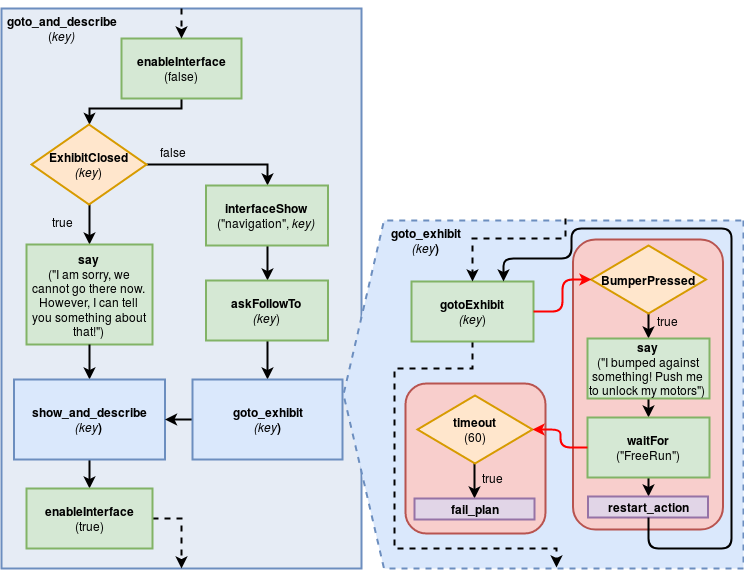
\includegraphics[width=1.05\linewidth]{imgs/lindsey_example_pnp.png}
            \end{column}
            \begin{column}{4cm}
              {\larger
                \begin{itemize}
                    \item Conditional plans made of \textbf{actions, conditions} and \textbf{Execution Rules}.
                    \item A PNP can be translated into a stochastic policy.
                \end{itemize}
              }
            \end{column}
        \end{columns}
    \end{block}
\end{frame}

\begin{frame}[shrink=10]{Robot Framework}
    \framesubtitle{Robot Management}
    \begin{columns}
    \begin{column}{0.65\textwidth}
        \begin{block}{User interface}
            \centering
            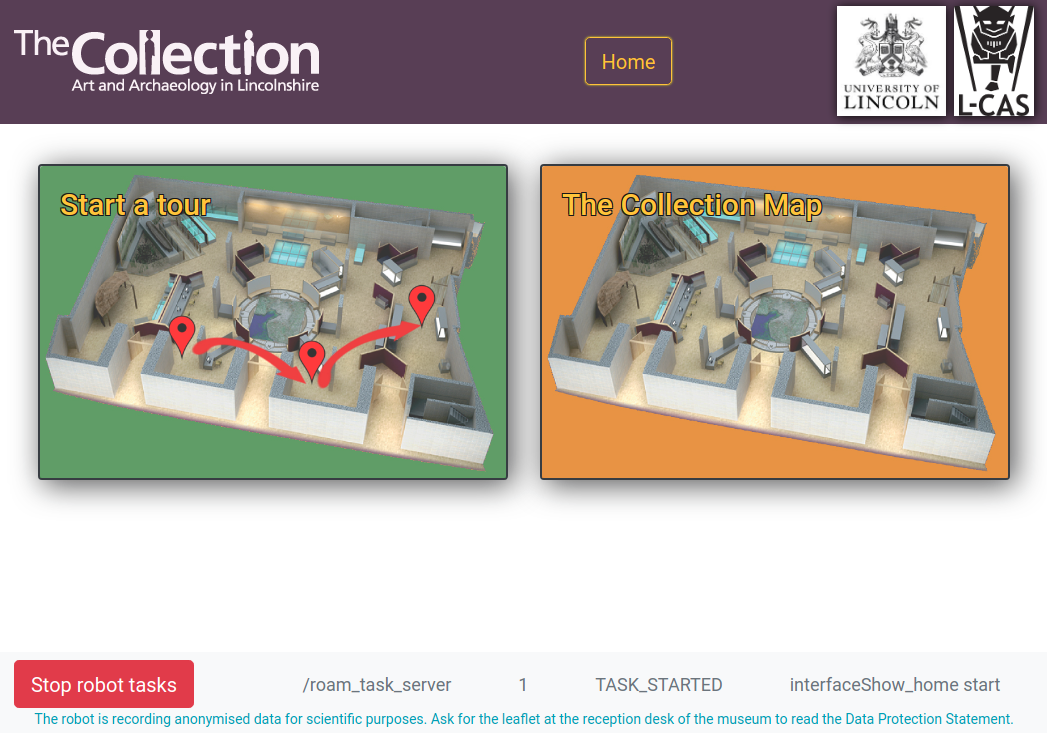
\includegraphics[width=0.31\linewidth]{imgs/home_page.png}
            \hspace{1pt}
            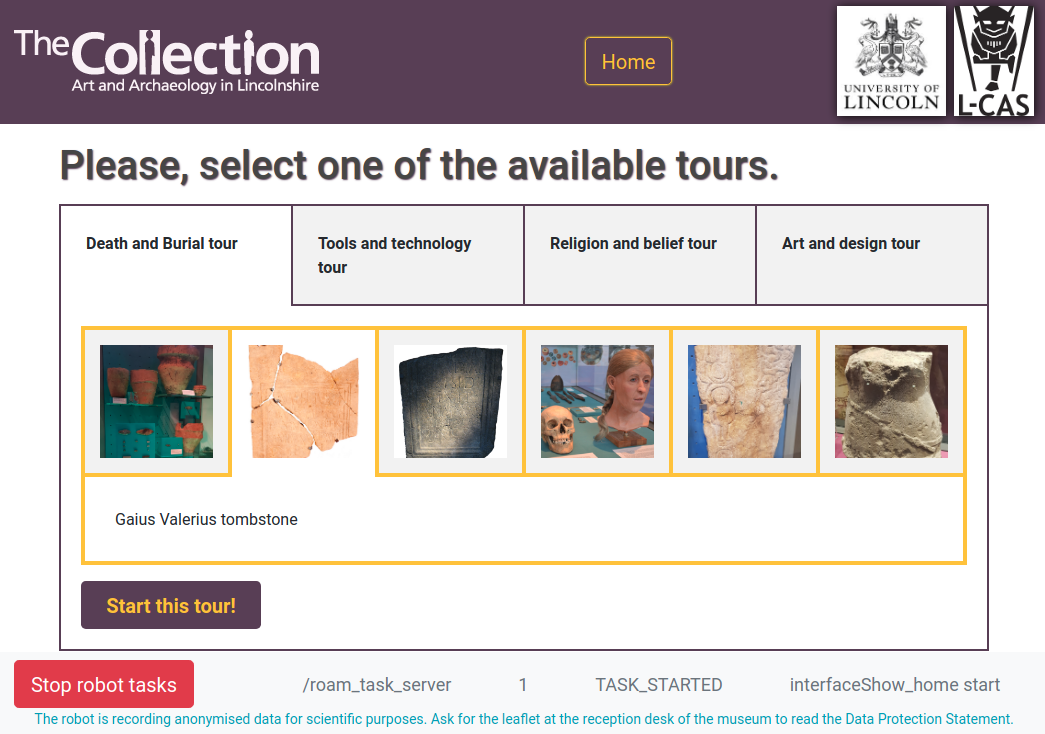
\includegraphics[width=0.31\linewidth]{imgs/tours_page.png}
            \hspace{1pt}
            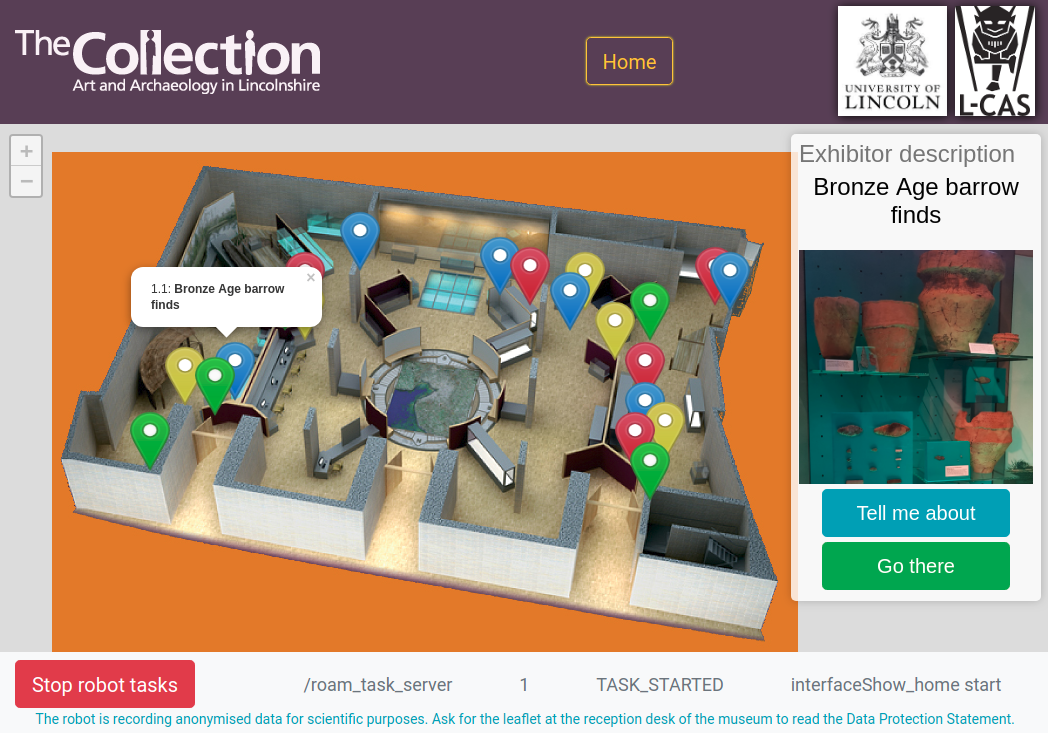
\includegraphics[width=0.31\linewidth]{imgs/map_page.png}
            {\\\scriptsize \url{https://github.com/laurencejbelliott/roswebcomponents}}
        \end{block}
        \vspace{-3pt}
        \begin{block}{Management interface}
            \centering
            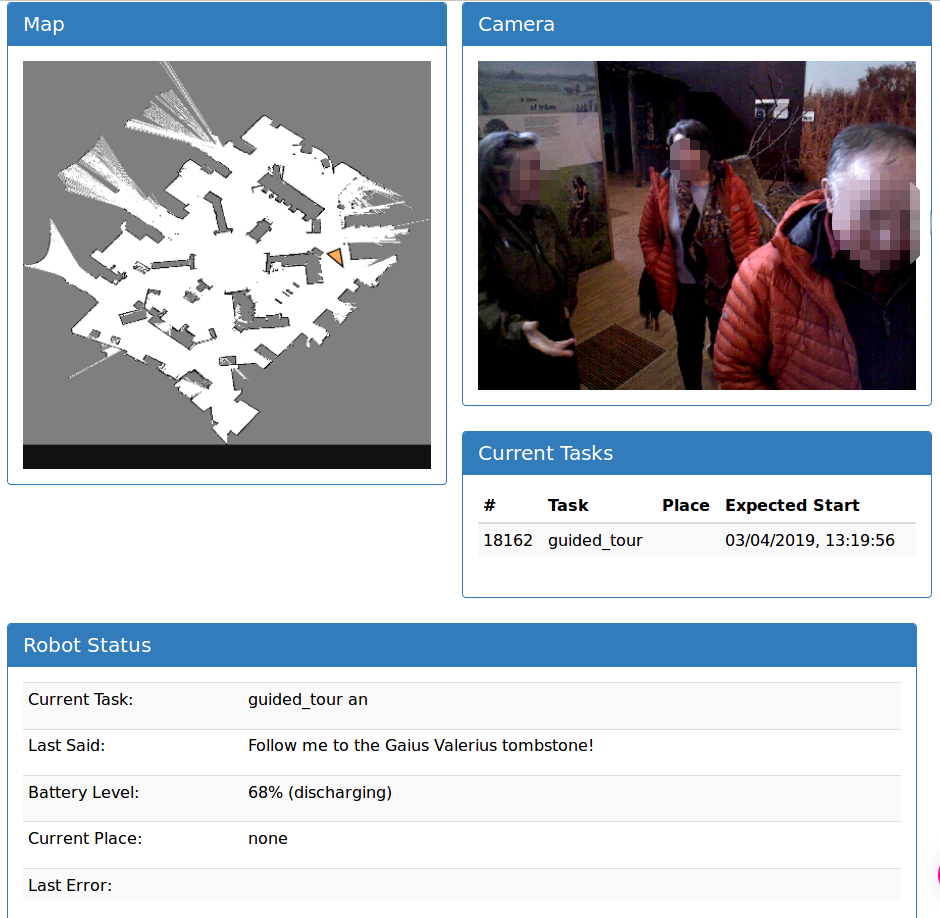
\includegraphics[width=0.31\linewidth]{imgs/admin_screen.png}
            \hspace{1pt}
            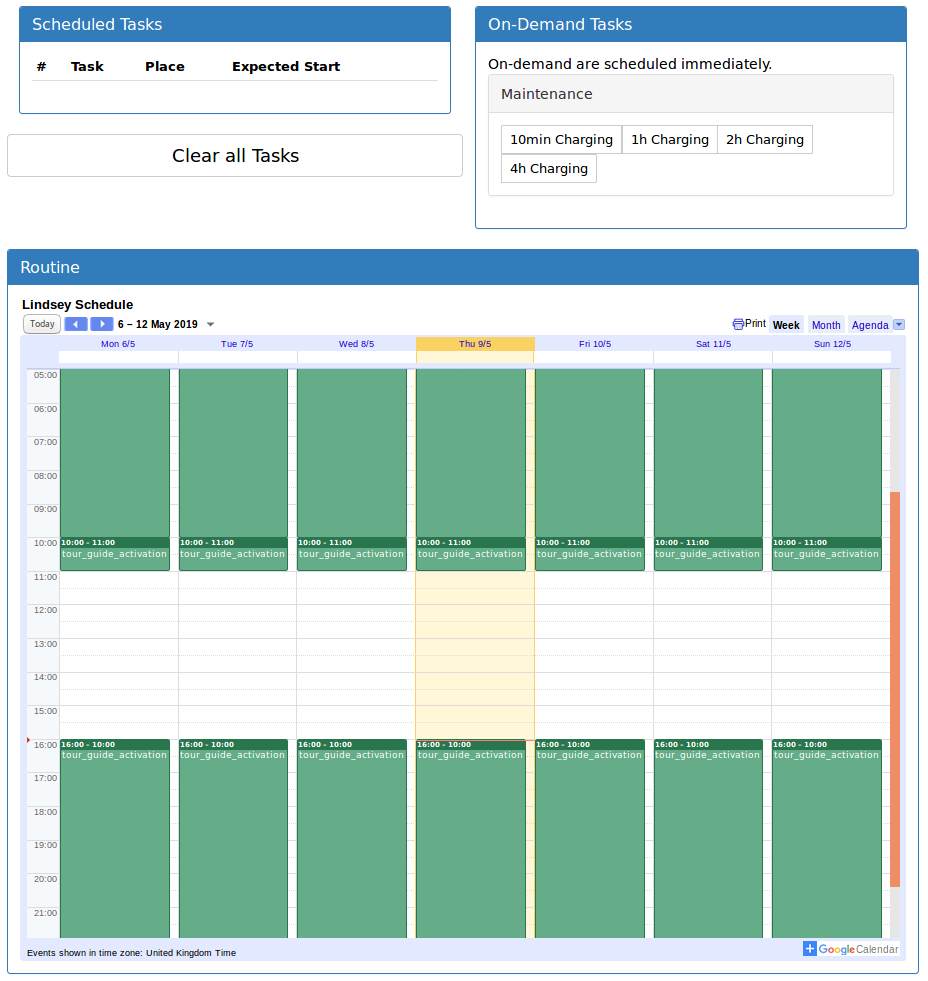
\includegraphics[width=0.31\linewidth]{imgs/admin_cal.png}
            \hspace{1pt}
            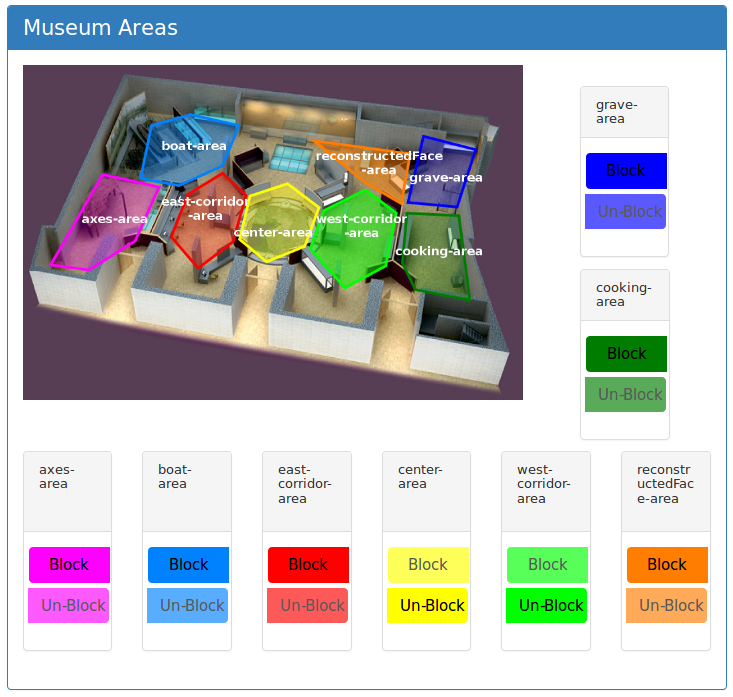
\includegraphics[width=0.31\linewidth]{imgs/admin_areas_cut.png}
        \end{block}
    \end{column}
    \begin{column}{0.35\textwidth}
        \vspace{-1cm}
        \begin{block}{Critical events notifications}
            \centering
            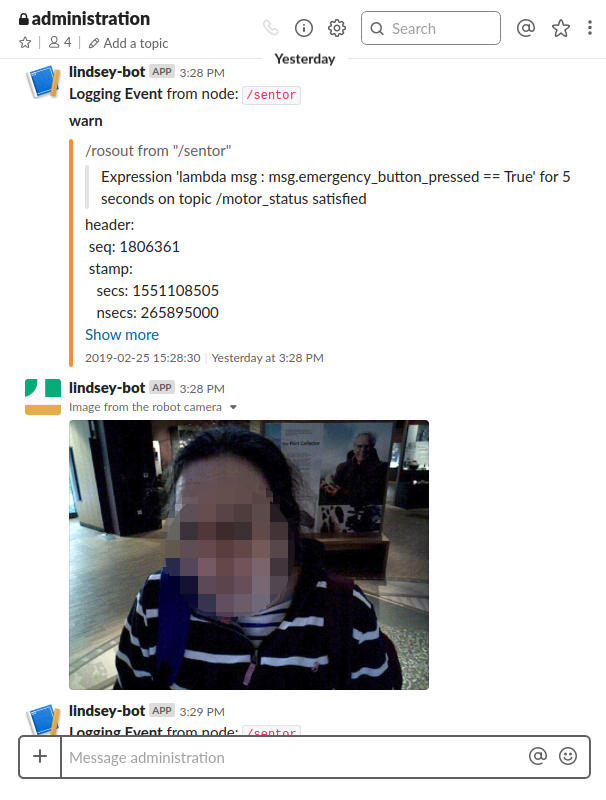
\includegraphics[width=0.9\linewidth]{imgs/notifications.png}
        \end{block}
    \end{column}
\end{columns}

\end{frame}


\begin{frame}[shrink=58]{Data Analysis}
    \vspace{-1cm}
    \begin{table}
        \caption{Long-Term Autonomy metrics.}
        \label{tab:metrics}
        \centering
        \begin{tabular}{|l|c|}
        \hline
        {Days of operation} & 103 days \\ \hline
        {Total distance travelled} & 299 km \\ \hline
        {Total tasks completed} & 8423 \\ \hline
        {TLS} & 26 days, 11 hours \\ \hline
        {A\%} & 74\% \\ \hline
        \end{tabular}
    \end{table}
    \vspace{7.8cm}
    \begin{table}
        \caption{Number of user demanded tasks with their duration.}
        \label{tab:dem_tasks}
        \centering
        \begin{tabular}{|l|c|c|c|c|c|}
        \hline
        \multicolumn{1}{|c|}{\textbf{Task}} & \multicolumn{1}{c|}{\textbf{Tot. demanded}} & \textbf{Average duration} & \textbf{Median duration} & \textbf{Shortest} & \textbf{Longest} \\ \hline
        % \hline
        \textit{{Guided tour}} & 2367 & 4.52 {[}min{]} & 3.13 {[}min{]} & 11 {[}sec{]} & 22.15 {[}min{]} \\ \hline
        \textit{{Go to exhibit and describe}} & 2379 & 1.87 {[}min{]} & 1.84 {[}min{]} & 8 {[}sec{]} & 30.79 {[}min{]} \\ \hline
        \textit{{Describe exhibit}} & 486 & 26.73 {[}sec{]} & 20.03 {[}sec{]} & 7.31 {[}sec{]} & 5.78 {[}min{]} \\ \hline
        \end{tabular}
    \end{table}
    
    \begin{textblock*}{4.4cm}(5mm, 26.5mm)
        \centering
        {\footnotesize How the tasks ends?}\\
        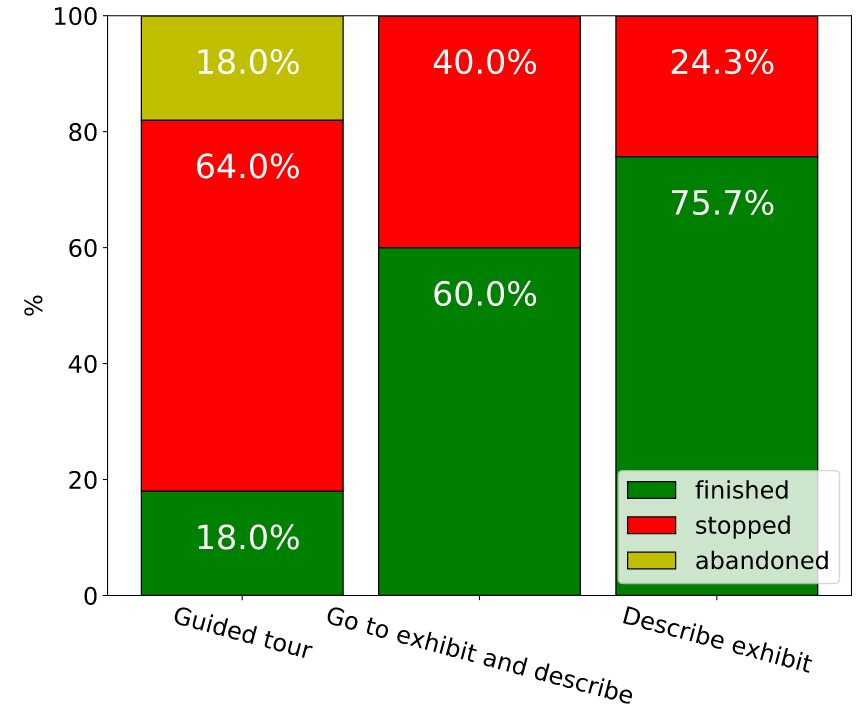
\includegraphics[width=\linewidth]{imgs/tasks_fate.png}
    \end{textblock*}
    \begin{textblock*}{5cm}(75mm, 30mm)
        \centering
        {\footnotesize What's the tours duration?}\\
        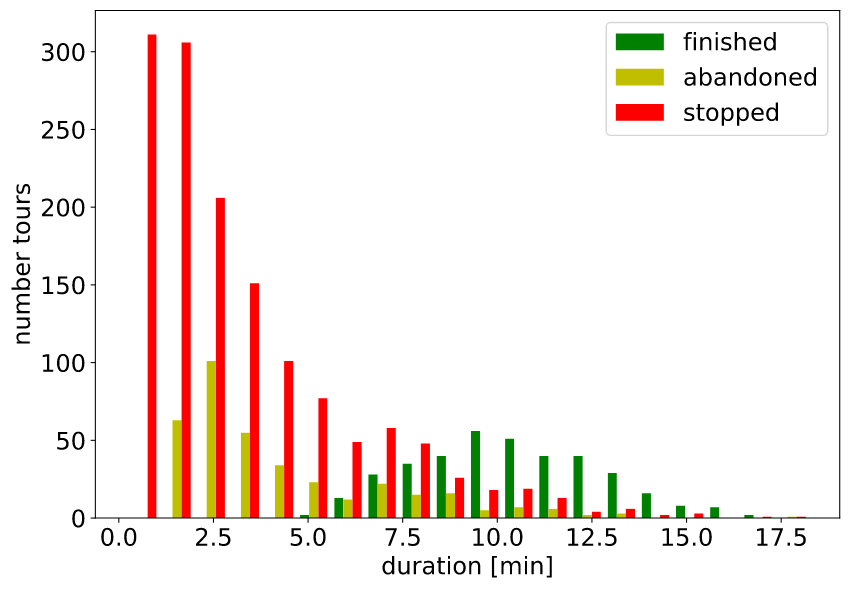
\includegraphics[width=\linewidth]{imgs/tours_duration.png}
    \end{textblock*}
\end{frame}

\begin{frame}[shrink=25]{Discussion}

    \begin{alertblock}{Engaged by the robot?}
        Engagement is easily started with Lindsey, but it is typically lost after 2 minutes.
    \end{alertblock}
    
    \begin{block}{How does a tour guide engage the public?}
    {\tiny From: Katie Best. Making museum tours better: Understanding what a guided tour really is and what a tour guide really does.}
        \begin{itemize}
            \item tours should not resemble monolithic lectures but they must be \textbf{interactive};
            \item guides should facilitate \textbf{audience contribution} through questions and answers;
            \item guides should seek to secure audience attention to inform and entertain them, encouraging them to \textbf{orient to the feature under consideration};
            \item the audience should not be considerate as a whole but the guide must take into account features of the single people, \textbf{personalizing the experience};
            \item technologists need to create non-human guides that have a similar level of \textbf{sensitivity to the audience} built-in.
        \end{itemize}
        
    \end{block}
\end{frame}

\section{Current Work \& Outlook}

\begin{frame}{Learning from engagement level}
    \begin{block}{}
        \lipsum[66]
    \end{block}
    \begin{center}
        \includegraphics[width=0.3\linewidth]{example-grid-100x100pt}
    \end{center}
\end{frame}

\begin{frame}{Engagement model}

    \begin{columns}
        \onslide*<1,3>{
            \begin{column}{0.5\linewidth}
                \begin{block}{Annotations}
                    % ṿideo is not shown here but it works with okular
                    \movie[width=\linewidth, height=0.8\linewidth, poster, autostart, borderwidth=2pt, loop, open, repeat, showcontrols=true]{Video not found, or use Okular}{vids/1558875962476119995_annotations.mp4} 
                \end{block}
            \end{column}     
        }
        \onslide*<1>{
            \begin{column}{0.5\linewidth}
                \begin{block}{}
                    \begin{itemize}
                        \item 3 Annotators
                        \item Continuous value for each frame in [0,1]
                        \item Inter-rater Spearman correlation $\rho$: 0.82
                    \end{itemize}
                \end{block}
            \end{column}
        }
        \onslide*<2>{
            \begin{column}{0.5\linewidth}
                % \begin{block}{}
                \hspace{-1.cm}
                \includegraphics[width=1.15\linewidth]{example-image-golden}
                % \end{block}
            \end{column}
        }
        \onslide*<2-3>{
            \begin{column}{0.5\linewidth}
                \begin{block}{Model predictions}
                    \movie[width=\linewidth, height=0.8\linewidth, poster, autostart, borderwidth=2pt, loop, open, repeat, showcontrols=true]{Video not found, or use Okular}{vids/1558875962476119995_predictions.mp4}
                \end{block}
            \end{column}
        }  
    \end{columns}


\end{frame}


\section*{The End}
\begin{frame}{Thank you for your attention!}
    \centering
    % this only works with okular pdf viewer...
    \movie[width=7cm, height=5cm, poster, autostart, start=76s, duration=5s, borderwidth=2pt, open, loop, repeat, showcontrols=true]{Video not found, or use Okular}{vids/lindsey_video.mp4}
\end{frame}
\end{document}






%%% Local Variables: 
%%% mode: latex
%%% TeX-PDF-mode: t 
%%% TeX-master: t
%%% End: 